\section{Data description}
\label{sec:description}

The dataset has three tiers: the raw recordings exactly as the phones exported them, the processed trajectories that most users will start from, and the map tiles and benchmark material that accompany the processed trajectories. \Cref{tab:devices} summarizes the recordings by device and \Cref{fig:tracks} shows where they were made.

\subsection{Repository layout}
\label{sec:layout}

The Zenodo record \todo{new Zenodo DOI} is organized as follows. \todo{confirm the final directory names once the record is assembled; the layout below is the one proposed for it.}

\begin{itemize}
\item \texttt{raw/<recording>/}: one directory per recording, named by its UTC start time as \texttt{YYYY-MM-DD\_hh-mm-ss}. All \numUtcNamed{} directory names match the epoch timestamp stored in their \texttt{Metadata.csv}. Each directory holds the Sensor Logger CSV exports (\Cref{sec:raw}).
\item \texttt{processed/<trajectory>.csv}: the \numTrajectories{} synchronized 10~Hz trajectories (\Cref{sec:processed}). A trajectory cut from a recording that had to be split carries a suffix \texttt{\_A}, \texttt{\_B}, \ldots{} in time order.
\item \texttt{processed/segments.json}: the segmentation manifest. It has one entry per recording or segment, giving the source recording, the start and end time in seconds from the start of the recording, the row count, and whether the segment was kept or why it was rejected.
\item \texttt{maps/<trajectory>\_\{relief,gravity,magnetic\}.nc}: map tiles cropped to each trajectory (\Cref{sec:maps}).
\item \texttt{benchmark/}: the scenario configurations and the per-trajectory error summaries behind \Cref{tab:benchmark}.
\end{itemize}

\begin{table}[t]
\centering
\caption{Recordings by device, as identified in each recording's \texttt{Metadata.csv}. \emph{Rec.}\ counts raw recordings and \emph{Traj.}\ counts processed trajectories; hours and distance are those of the processed trajectories. \emph{GNSS file} is the raw file that the processed GNSS columns are taken from: \texttt{LocationGps} is Android's GNSS-only provider and \texttt{Location} is the platform's fused location service.}
\label{tab:devices}
\small
\begin{tabular}{llrrrrl}
\toprule
Device (as logged) & OS & Rec. & Traj. & Hours & km & GNSS file \\
\midrule
Pixel 6a & Android & 5 & 5 & 9.4 & 593 & \texttt{LocationGps} \\
SM-S921U & Android & 2 & 2 & 3.0 & 228 & \texttt{Location} \\
Pixel 9 Pro & Android & 12 & 13 & 26.9 & 2{,}159 & \texttt{LocationGps} \\
SM-A146U & Android & 2 & 1 & 0.2 & 13 & \texttt{Location} \\
Pixel 9 Pro XL & Android & 2 & 2 & 3.7 & 294 & \texttt{LocationGps} \\
iPhone 12 mini & iOS & 5 & 3 & 10.3 & 956 & \texttt{Location} \\
iPhone 13 mini & iOS & 1 & 1 & 1.8 & 96 & \texttt{Location} \\
\midrule
Total & & 29 & 27 & 55.3 & 4{,}338 & \\
\bottomrule
\end{tabular}

\end{table}

\begin{figure}[t]
\centering
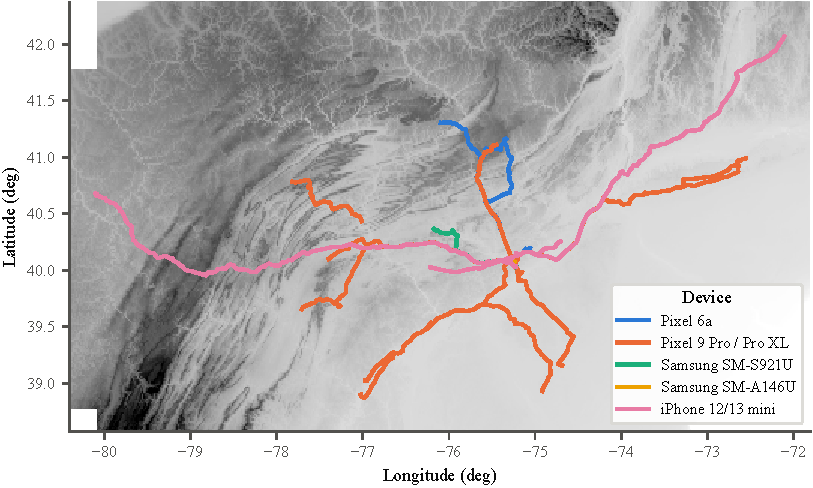
\includegraphics[width=\linewidth]{figures/fig_tracks.pdf}
\caption{GNSS tracks of the \numTrajectories{} processed trajectories, colored by device family, over the 15 arc-second relief tiles that accompany them (darker is higher). The single Samsung SM-A146U trajectory is short and lies under other tracks near 40.1\textdegree{}N, 75.3\textdegree{}W.}
\label{fig:tracks}
\end{figure}

\subsection{Raw recordings}
\label{sec:raw}

There are \numRawRecordings{} raw recordings, made between \numRawFirst{} and \numRawLast{} with Sensor Logger versions 1.18.0 to 1.48.0 \citep{sensorlogger}. Together they hold \numRawGB~GB in about \numRawRowsMillion{} million rows and span \numRawHours~h of wall-clock time. One recording (\texttt{2025-06-13\_14-55-15}) contains no sensor data. Every sensor file has the columns \texttt{time}, the UTC epoch time in nanoseconds, and \texttt{seconds\_elapsed}, the time since the recording started, followed by its measured quantities. Three-axis sensors give \texttt{x}, \texttt{y} and \texttt{z} in the phone's body frame as reported by the operating system. \texttt{Metadata.csv} records the device model, platform, application version, the list of enabled sensors, their requested sampling interval in milliseconds, and whether Sensor Logger's cross-platform unit standardization was on.

The files present depend on the platform and the application version. All recordings with data have \texttt{Gyroscope}, \texttt{Accelerometer}, \texttt{Gravity}, \texttt{Magnetometer}, \texttt{Orientation} and \texttt{Location}. Android recordings add \texttt{TotalAcceleration} (specific force including gravity). Recordings from 2025 onward add \texttt{GyroscopeUncalibrated}, \texttt{AccelerometerUncalibrated}, \texttt{MagnetometerUncalibrated} and \texttt{Compass}. Pixel recordings add the separate GNSS (\texttt{LocationGps}) and network (\texttt{LocationNetwork}) location providers, and Pixel 9 Pro recordings also add \texttt{GameOrientation} and \texttt{GeomagneticOrientation}. On both platforms \texttt{Accelerometer} is linear acceleration, with gravity removed. \numNoBaroRecordings{} iPhone recordings (\numNoBaroHours~h) have no barometer data and are released in raw form only. \Cref{tab:channels} lists the median sampling rate of each channel by device family, measured from the timestamps.

\begin{table}[t]
\centering
\caption{Sensor channels. Rates are the median, over the recordings of each device family that enter the processed set, of each recording's median sampling rate (Hz) in the raw files; every channel is resampled to 10~Hz in the processed files. Sensor Logger requested a 10~ms interval for all inertial channels and left the barometer and location at their defaults. (a)~On iOS, where there is no \texttt{TotalAcceleration}, specific force is formed as \texttt{Accelerometer} plus \texttt{Gravity}. (b)~\texttt{Location} where \texttt{LocationGps} is absent (\Cref{tab:devices}). Processed column names are abbreviated; \Cref{sec:processed} lists them in full with their units.}
\label{tab:channels}
\footnotesize
\setlength{\tabcolsep}{2.5pt}
\begin{tabular}{llllrrrrr}
\toprule
Channel & Raw file & Columns & Unit & \rotatebox{90}{Pixel 6a} & \rotatebox{90}{Pixel 9 Pro / Pro XL} & \rotatebox{90}{Samsung SM-S921U} & \rotatebox{90}{Samsung SM-A146U} & \rotatebox{90}{iPhone 12/13 mini} \\
\midrule
Specific force & \texttt{TotalAcceleration}\textsuperscript{a} & \texttt{acc\_*} & m\,s\(^{-2}\) & 56 & 100 & 60 & 100 & 101 \\
Angular rate & \texttt{Gyroscope} & \texttt{gyro\_*} & rad\,s\(^{-1}\) & 56 & 100 & 60 & 100 & 101 \\
Magnetic field & \texttt{Magnetometer} & \texttt{mag\_*} & \(\mu\)T & 100 & 100 & 100 & 100 & 101 \\
Gravity (fused) & \texttt{Gravity} & \texttt{grav\_*} & m\,s\(^{-2}\) & 56 & 100 & 100 & 100 & 101 \\
Attitude (fused) & \texttt{Orientation} & \texttt{q*}, \texttt{roll}, \ldots & --, rad & 56 & 100 & 100 & 100 & 101 \\
Pressure & \texttt{Barometer} & \texttt{pressure}, \ldots & hPa, m & 50 & 40 & 25 & 10 & 1 \\
GNSS fix & \texttt{LocationGps}\textsuperscript{b} & \texttt{latitude}, \ldots & see text & 1 & 1 & 1 & 1 & 1 \\
\bottomrule
\end{tabular}

\end{table}

\subsection{Processed trajectories}
\label{sec:processed}

The \numTrajectories{} processed trajectories hold \numRows{} rows at 10~Hz. \Cref{tab:trajectories} lists them. They last from \numMinHours~h to \numMaxHours~h and cover \numMinKm~km to \numMaxKm~km, for \numTotalHours~h and \numTotalKm~km in total. The median GNSS speed is \numMedianSpeed~km/h, so most of the driving is on highways. Each file has the following columns.
\begin{itemize}
\item \texttt{time}: ISO 8601 timestamp in UTC, at the start of each 0.1~s bin.
\item \texttt{latitude}, \texttt{longitude} (degrees, WGS84), \texttt{altitude} (m, as reported by the location service), \texttt{speed} (m/s), \texttt{bearing} (degrees from north), and the receiver's reported \texttt{horizontalAccuracy} (m), \texttt{verticalAccuracy} (m), \texttt{speedAccuracy} (m/s) and \texttt{bearingAccuracy} (degrees). These columns are filled only in rows that contain a GNSS fix and are empty elsewhere.
\item \texttt{acc\_x}, \texttt{acc\_y}, \texttt{acc\_z}: specific force in the body frame (m/s\(^2\)), including gravity, so that a phone at rest reads about \(+9.8\)~m/s\(^2\) along its upward axis.
\item \texttt{gyro\_x}, \texttt{gyro\_y}, \texttt{gyro\_z}: angular rate (rad/s), as calibrated by the operating system.
\item \texttt{mag\_x}, \texttt{mag\_y}, \texttt{mag\_z}: magnetic flux density (\(\mu\)T), with the operating system's hard-iron correction applied (\Cref{sec:magnetometer}).
\item \texttt{grav\_x}, \texttt{grav\_y}, \texttt{grav\_z}: the operating system's fused gravity estimate (m/s\(^2\); \Cref{sec:gravity}).
\item \texttt{qw}, \texttt{qx}, \texttt{qy}, \texttt{qz} and \texttt{roll}, \texttt{pitch}, \texttt{yaw} (rad): the operating system's fused attitude.
\item \texttt{pressure} (hPa) and \texttt{relativeAltitude} (m, change since the recording began, derived from pressure).
\end{itemize}
The GNSS columns hold \numFixes{} fixes, a median of \numMedianFixRate{} fixes per second per trajectory, and they are never interpolated: in about nine rows out of ten they are empty. The inertial columns are complete in every row. iOS phones deliver pressure at about 1~Hz, so on those trajectories only a median of \numIosBaroFraction\% of rows carry a pressure value.

\begin{table}[p]
\centering
\caption{The processed trajectories. \emph{Speed} is the median GNSS speed, \emph{Fixes} the number of rows with a GNSS fix, and \emph{Fix rate} the fixes per second of trajectory. \(\sigma_h\), \(\sigma_v\) and \(\sigma_s\) are the medians of the receiver's reported horizontal, vertical and speed accuracy over those fixes. Distance is the summed great-circle distance between successive fixes.}
\label{tab:trajectories}
\scriptsize
\setlength{\tabcolsep}{3pt}
\begin{tabular}{llrrrrrrrr}
\toprule
Trajectory & Device & h & km & \makecell{Speed\\(km/h)} & Fixes & \makecell{Fix\\rate (Hz)} & \makecell{\(\sigma_h\)\\(m)} & \makecell{\(\sigma_v\)\\(m)} & \makecell{\(\sigma_s\)\\(m/s)} \\
\midrule
2023-08-04\_21-47-58 & Pixel 6a & 2.45 & 158.3 & 87 & 8{,}034 & 0.91 & 2.0 & 2.5 & 0.18 \\
2023-08-06\_14-48-05 & Pixel 6a & 2.48 & 169.1 & 77 & 8{,}920 & 1.00 & 2.0 & 2.4 & 0.17 \\
2023-08-09\_12-47-42 & Pixel 6a & 1.45 & 32.1 & 3 & 5{,}174 & 0.99 & 2.6 & 3.1 & 0.23 \\
2023-08-09\_16-37-41 & Pixel 6a & 0.72 & 41.0 & 63 & 2{,}579 & 1.00 & 2.2 & 2.7 & 0.20 \\
2024-06-20\_16-55-50 & Pixel 6a & 2.34 & 192.3 & 99 & 8{,}391 & 1.00 & 7.8 & 3.0 & 0.23 \\
2025-03-01\_15-04-26 & SM-S921U & 1.51 & 114.2 & 84 & 5{,}457 & 1.00 & 3.8 & 1.3 & 0.08 \\
2025-03-01\_16-46-39 & SM-S921U & 1.49 & 113.6 & 83 & 5{,}386 & 1.00 & 3.8 & 1.3 & 0.08 \\
2025-06-11\_20-34-24\_A & Pixel 9 Pro & 0.11 & 2.1 & 16 & 411 & 1.00 & 6.6 & 3.0 & 0.46 \\
2025-06-14\_21-17-02 & SM-A146U & 0.16 & 12.7 & 2 & 197 & 0.34 & 12.2 & 0.7 & 0.39 \\
2025-06-18\_15-09-25 & Pixel 9 Pro XL & 1.48 & 148.9 & 111 & 5{,}248 & 0.98 & 8.2 & 3.0 & 0.38 \\
2025-06-18\_16-52-32 & Pixel 9 Pro XL & 2.20 & 144.9 & 74 & 7{,}916 & 1.00 & 5.1 & 2.0 & 0.20 \\
2025-06-27\_11-54-35 & iPhone 12 mini & 4.95 & 402.3 & 99 & 17{,}767 & 1.00 & 10.0 & 19.0 & 0.20 \\
2025-07-04\_17-24-46 & Pixel 9 Pro & 1.74 & 137.4 & 94 & 6{,}227 & 0.99 & 6.6 & 2.0 & 0.25 \\
2025-07-05\_20-59-22 & Pixel 9 Pro & 2.51 & 138.5 & 55 & 9{,}017 & 1.00 & 7.1 & 3.0 & 0.31 \\
2025-07-08\_14-12-53 & iPhone 13 mini & 1.85 & 96.2 & 55 & 6{,}658 & 1.00 & 2.5 & 3.0 & 1.56 \\
2025-07-11\_13-33-16 & Pixel 9 Pro & 1.66 & 136.2 & 98 & 5{,}961 & 1.00 & 1.5 & 1.0 & 0.12 \\
2025-07-18\_23-13-43 & Pixel 9 Pro & 1.55 & 152.1 & 109 & 5{,}526 & 0.99 & 1.5 & 1.0 & 0.13 \\
2025-07-31\_23-36-03 & Pixel 9 Pro & 3.74 & 304.6 & 88 & 13{,}450 & 1.00 & 1.5 & 1.0 & 0.13 \\
2025-08-03\_18-15-59 & Pixel 9 Pro & 4.14 & 298.2 & 84 & 14{,}892 & 1.00 & 1.5 & 1.0 & 0.14 \\
2025-09-26\_19-03-38 & iPhone 12 mini & 4.59 & 497.2 & 123 & 16{,}505 & 1.00 & 5.0 & 9.5 & 0.20 \\
2025-09-27\_12-54-35 & Pixel 9 Pro & 2.26 & 213.0 & 109 & 8{,}136 & 1.00 & 2.0 & 1.0 & 0.14 \\
2025-09-27\_18-10-16 & iPhone 12 mini & 0.76 & 56.3 & 89 & 2{,}731 & 1.00 & 10.0 & 19.0 & 0.20 \\
2025-09-28\_20-23-16 & Pixel 9 Pro & 3.33 & 286.3 & 99 & 11{,}996 & 1.00 & 2.0 & 1.0 & 0.13 \\
2025-11-09\_17-34-01\_A & Pixel 9 Pro & 1.07 & 108.0 & 106 & 3{,}854 & 1.00 & 1.5 & 1.0 & 0.12 \\
2025-11-09\_17-34-01\_B & Pixel 9 Pro & 0.16 & 1.1 & 0 & 559 & 1.00 & 2.0 & 1.0 & 0.01 \\
2025-11-09\_17-34-01\_C & Pixel 9 Pro & 1.40 & 141.8 & 115 & 5{,}020 & 1.00 & 2.0 & 1.0 & 0.31 \\
2025-11-16\_16-08-14 & Pixel 9 Pro & 3.23 & 239.1 & 90 & 11{,}510 & 0.99 & 2.0 & 1.0 & 0.14 \\
\midrule
Total & & 55.3 & 4{,}338 & & 197{,}522 & & & & \\
Median & & 1.74 & 141.8 & 88 & 6{,}227 & 1.00 & 2.5 & 2.0 & 0.20 \\
\bottomrule
\end{tabular}

\end{table}

\subsection{Map tiles}
\label{sec:maps}

Each processed trajectory comes with three NetCDF grids cropped to its padded bounding box. Each grid has variables \texttt{lat}, \texttt{lon} (degrees) and \texttt{z}: relief at 15 arc-seconds (m; SRTM15+, \citealp{tozer2019srtm15}), free-air gravity anomaly at 1 arc-minute (mGal; \citealp{SANDWELL20211059}) and magnetic anomaly at 3 arc-minutes (nT; WDMAM, \citealp{wdmam}). They were fetched through the Generic Mapping Tools remote datasets \citep{wessel2019gmt}, are provided for convenience, and remain subject to their originators' terms.
